As mentioned in \ref{sec:Introduction:Problem Definition}, our solution must design a feasible trajectory for each robot to transport the payload and create an adaptive control law for trajectory execution. The proposed system architecture is depicted in \ref{fig:Proposed Approach: System Architecture : System Architecture}. Unlike classical path and trajectory planning approaches, our method introduces a closed-loop system, described as a continuous planning system, as detailed in~\cite{durfee1999survey}. This approach is particularly suited to dynamic environments where changes may occur due to unknown agents. 

It is important to clarify the use of the term "continuous planning" in this context. The term refers to the state domain rather than the time domain. While the system operates in a discrete time domain, planning occurs continuously in the state domain. This ensures that the path is reevaluated whenever necessary, allowing for updates to the trajectory based on environmental or operational changes.

The primary advantage of incorporating feedback loops not only in the control phase but also in trajectory generation is the system's ability to adapt and correct model errors dynamically. Furthermore, it facilitates payload transportation even in the absence of precise mechanical parameters, resulting in a robust system capable of functioning across diverse scenarios. Such robustness is not achievable with classical planning approaches, where the generated trajectory remains static during execution.

\begin{figure}[H]
    \centering
    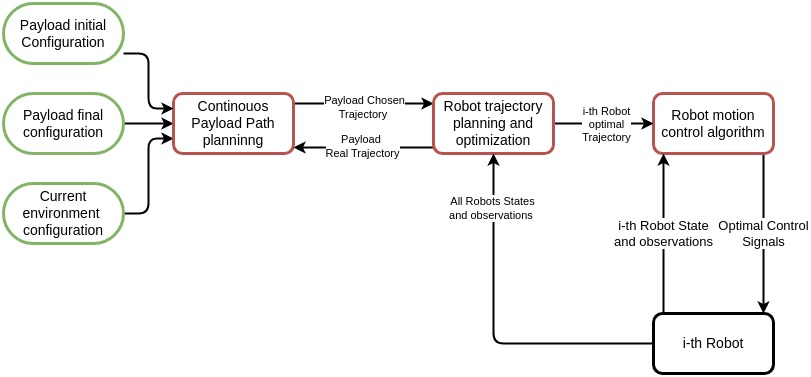
\includegraphics[width=0.7\textwidth]{Images/Propposed Aproach/system Architecture.png}
    \caption{Proposed high-level system architecture. Data required in each stage is shown in green, while the stages are depicted in red. Arrows represent the data flow between stages.}
    \label{fig:Proposed Approach: System Architecture : System Architecture}
\end{figure}

Feedback loops in this system can be managed in two distinct ways: fixed time step or event-driven. In the fixed time step approach, the system periodically checks whether the trajectory requires replanning after a predefined interval. If replanning is necessary, the trajectory module updates the path, and the system uses the new reference. Conversely, in the event-driven approach, trajectory replanning is triggered by specific events, such as obstacle detection or significant deviation between the reference and actual positions.

Each method has its advantages, but certain constraints must be observed. If a preceding stage employs a fixed time step, all subsequent stages must also adopt a fixed time step. Furthermore, the control algorithm always operates on a fixed time step. These considerations result in the possible configurations outlined in Table~\ref{tab:Proposed Approach: System Architechture}. The final configuration will be determined in the final report after additional testing to identify the optimal approach and establish a performance baseline.

\begin{table}[H]
    \centering
    \resizebox{0.8\textwidth}{!}{%
    \begin{tabular}{ccc}
    \hline
        \textbf{Configuration} & \textbf{Payload Path Planning} & \textbf{Robots Trajectory Planning} \\ \hline
        \textbf{Scenario 1} & Event-Driven & Event-Driven \\ 
        \textbf{Scenario 2} & Event-Driven & Fixed Rate \\ 
        \textbf{Scenario 3} & Fixed Rate & Fixed Rate \\ \hline
    \end{tabular}
    }
    \caption{Possible feedback architectures for the proposed system.}
    \label{tab:Proposed Approach: System Architechture}
\end{table}
